In a simple AM radio, a coil ($L = \LrO$) and a variable capacitor form a parallel resonant circuit at the antenna. Its impedance is large only near its resonance frequency: there, the signal of a station builds up a voltage across the circuit, while all others are short-circuited. Turning the knob changes $C$. The graph shows the measured impedance of the circuit.

\begin{center}
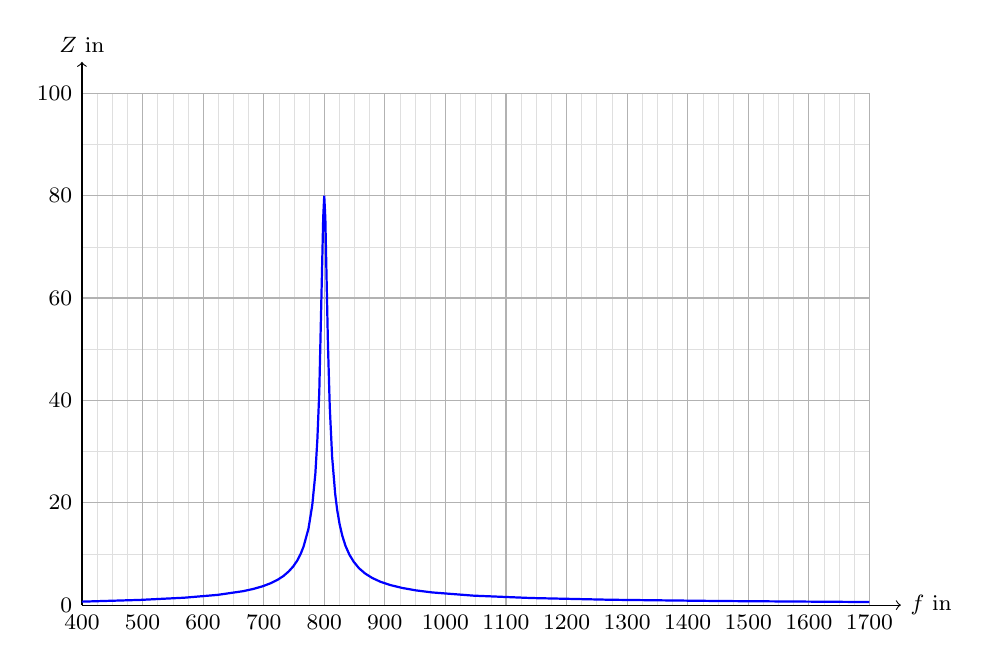
\begin{tikzpicture}[font=\footnotesize]
 \draw[gray!25, very thin] (0.192,0) -- (0.192,6.500) (0.385,0) -- (0.385,6.500) (0.577,0) -- (0.577,6.500) (0.962,0) -- (0.962,6.500) (1.154,0) -- (1.154,6.500) (1.346,0) -- (1.346,6.500) (1.731,0) -- (1.731,6.500) (1.923,0) -- (1.923,6.500) (2.115,0) -- (2.115,6.500) (2.500,0) -- (2.500,6.500) (2.692,0) -- (2.692,6.500) (2.885,0) -- (2.885,6.500) (3.269,0) -- (3.269,6.500) (3.462,0) -- (3.462,6.500) (3.654,0) -- (3.654,6.500) (4.038,0) -- (4.038,6.500) (4.231,0) -- (4.231,6.500) (4.423,0) -- (4.423,6.500) (4.808,0) -- (4.808,6.500) (5.000,0) -- (5.000,6.500) (5.192,0) -- (5.192,6.500) (5.577,0) -- (5.577,6.500) (5.769,0) -- (5.769,6.500) (5.962,0) -- (5.962,6.500) (6.346,0) -- (6.346,6.500) (6.538,0) -- (6.538,6.500) (6.731,0) -- (6.731,6.500) (7.115,0) -- (7.115,6.500) (7.308,0) -- (7.308,6.500) (7.500,0) -- (7.500,6.500) (7.885,0) -- (7.885,6.500) (8.077,0) -- (8.077,6.500) (8.269,0) -- (8.269,6.500) (8.654,0) -- (8.654,6.500) (8.846,0) -- (8.846,6.500) (9.038,0) -- (9.038,6.500) (9.423,0) -- (9.423,6.500) (9.615,0) -- (9.615,6.500) (9.808,0) -- (9.808,6.500);
 \draw[gray!25, very thin] (0,0.650) -- (10.000,0.650) (0,1.950) -- (10.000,1.950) (0,3.250) -- (10.000,3.250) (0,4.550) -- (10.000,4.550) (0,5.850) -- (10.000,5.850);
 \draw[gray!60, thin] (0.000,0) -- (0.000,6.500) (0.769,0) -- (0.769,6.500) (1.538,0) -- (1.538,6.500) (2.308,0) -- (2.308,6.500) (3.077,0) -- (3.077,6.500) (3.846,0) -- (3.846,6.500) (4.615,0) -- (4.615,6.500) (5.385,0) -- (5.385,6.500) (6.154,0) -- (6.154,6.500) (6.923,0) -- (6.923,6.500) (7.692,0) -- (7.692,6.500) (8.462,0) -- (8.462,6.500) (9.231,0) -- (9.231,6.500) (10.000,0) -- (10.000,6.500);
 \draw[gray!60, thin] (0,0.000) -- (10.000,0.000) (0,1.300) -- (10.000,1.300) (0,2.600) -- (10.000,2.600) (0,3.900) -- (10.000,3.900) (0,5.200) -- (10.000,5.200) (0,6.500) -- (10.000,6.500);
 \node[below] at (0.000,0) {400};
 \node[below] at (0.769,0) {500};
 \node[below] at (1.538,0) {600};
 \node[below] at (2.308,0) {700};
 \node[below] at (3.077,0) {800};
 \node[below] at (3.846,0) {900};
 \node[below] at (4.615,0) {1000};
 \node[below] at (5.385,0) {1100};
 \node[below] at (6.154,0) {1200};
 \node[below] at (6.923,0) {1300};
 \node[below] at (7.692,0) {1400};
 \node[below] at (8.462,0) {1500};
 \node[below] at (9.231,0) {1600};
 \node[below] at (10.000,0) {1700};
 \node[left] at (0,0.000) {0};
 \node[left] at (0,1.300) {20};
 \node[left] at (0,2.600) {40};
 \node[left] at (0,3.900) {60};
 \node[left] at (0,5.200) {80};
 \node[left] at (0,6.500) {100};
 \draw[->] (0,0) -- (10.400,0) node[right] {$f$ in \si{\kilo\hertz}};
 \draw[->] (0,0) -- (0,6.900) node[above] {$Z$ in \si{\kilo\ohm}};
 \draw[thick, blue] plot coordinates {(0.000,0.044) (0.738,0.066) (1.299,0.094) (1.724,0.130) (2.047,0.177) (2.179,0.206) (2.294,0.239) (2.394,0.277) (2.482,0.320) (2.559,0.370) (2.625,0.427) (2.684,0.492) (2.734,0.566) (2.777,0.649) (2.815,0.745) (2.877,0.972) (2.925,1.271) (2.964,1.668) (2.990,2.111) (3.014,2.707) (3.064,4.925) (3.077,5.200) (3.091,4.906) (3.124,3.314) (3.147,2.518) (3.177,1.884) (3.216,1.412) (3.241,1.211) (3.271,1.033) (3.306,0.882) (3.347,0.752) (3.396,0.642) (3.451,0.551) (3.517,0.470) (3.594,0.403) (3.686,0.345) (3.792,0.296) (3.919,0.254) (4.067,0.218) (4.242,0.187) (4.447,0.161) (4.974,0.120) (5.703,0.090) (6.708,0.068) (8.095,0.052) (10.000,0.039)};
\end{tikzpicture}
\end{center}

\begin{abcliste}
\abc To which frequency $f_0$ is the radio tuned?
\abc What is $C$ now?
\abc Which capacitance $C_2$ tunes the radio to a station at \fbO?
\end{abcliste}
